\documentclass[conference]{IEEEtran}
\usepackage{graphicx}
\usepackage{booktabs}
\usepackage{amsmath}
\usepackage{amssymb}
\usepackage{cite}
\usepackage{placeins}
\usepackage{caption}
\usepackage{subcaption}
\usepackage{multirow}
\usepackage{tabularx}
\usepackage{dblfloatfix}
\usepackage{etoolbox}
\usepackage{float}
\usepackage[hidelinks]{hyperref}

\makeatletter
\patchcmd{\thebibliography}{\section*{\refname}}{\section*{\centering\refname}}{}{}
\makeatother

\graphicspath{{figures/}}

\setlength{\textfloatsep}{6pt plus 2pt minus 2pt}
\setlength{\floatsep}{4pt plus 2pt minus 2pt}
\setlength{\intextsep}{6pt plus 2pt minus 2pt}
\captionsetup{font=small,labelfont=bf,skip=3pt}
\captionsetup[subfigure]{font=scriptsize,skip=2pt}

\newcommand{\ie}{\textit{i.e.}}
\newcommand{\eg}{\textit{e.g.}}

\title{Fixed Geometry, Not Learned Residuals:\\
Exposing Ego-Motion Shortcuts in Sensor-Free Pedestrian Trajectory and Intent Prediction}

\author{\IEEEauthorblockN{}
\IEEEauthorblockA{}}

\begin{document}
\maketitle

% ======================================================================
\begin{abstract}
Cameras mounted on moving vehicles record every pedestrian's image-plane trajectory as a mixture of pedestrian motion and camera motion, so a person standing still still appears to drift across the frame. This paper proposes and validates a sensor-free, position-dependent ego-motion compensation method for pedestrian trajectory and intent prediction. It also introduces a standing-pedestrian variance gate, a physical validity test that any such compensation method must pass before its downstream results can be trusted. We compare a learned multi-agent residual module, trained under three supervision regimes, against a fixed offline compensator that estimates a full affine transform from ORB feature matches and applies it at each agent's own image position rather than as a single global shift. All three learned variants fail the variance gate, passing fewer than 1\% of diagnostic windows, despite one variant showing a superficially plausible correlation of 0.30 with ground-truth vehicle speed. The fixed affine method passes 93.1\% of PIE windows and 96.9\% of JAAD windows. It is trajectory-neutral on PIE, with ADE changing from 60.8 to 60.5 pixels, a difference of 0.5\%, using zero ego-motion sensor at inference. On JAAD, where no such sensor exists at all, it reduces ADE by 25\%, from 83.1 to 62.7 pixels. A further finding is that intent-prediction accuracy rises monotonically with the amount of ego-motion information available to the model, with AUC of 0.80, 0.89, and 0.93 across three conditions, indicating that a meaningful share of reported intent accuracy reflects a camera-motion shortcut rather than genuine pedestrian-intent understanding.
\end{abstract}

\begin{IEEEkeywords}
pedestrian trajectory prediction, pedestrian intent prediction, ego-motion compensation, ORB, RANSAC, affine stabilisation, variance gate, causal shortcuts, JAAD, PIE
\end{IEEEkeywords}

% ======================================================================
\section{Introduction}

Road traffic crashes kill more than 1.19~million people every year, and
pedestrians alone account for 23\% of these deaths, with vulnerable road
users overall making up 53\% of the global total~\cite{who2023roadsafety}.
Reducing this toll is one of the central motivations behind autonomous and
driver-assistance systems, but a vehicle can only act on this motivation
if it can anticipate what a nearby pedestrian is about to do with enough
lead time to respond. Predicting a pedestrian's future position and
crossing intention from vehicle-mounted video has therefore become an
active research problem, building on a broader trajectory-prediction
literature developed first in pedestrian-only and social
settings~\cite{alahi2016sociallstm,gupta2018socialgan}, and later
extended to the specific and harder case of a single moving camera
mounted on a vehicle.

The title of this paper names the three things we found while studying
that harder case. A camera mounted on a moving vehicle records every
object's position purely in image coordinates, and those coordinates mix
two unrelated signals: how the pedestrian actually moved, and how the
vehicle's own motion shifted the camera's viewpoint. A pedestrian
standing motionless on the footpath still drifts steadily across the
frame simply because the vehicle advanced. ``Fixed Geometry'' refers to
our central finding that a classical, offline geometric estimate of this
camera-induced shift is what actually works. ``Not Learned Residuals''
refers to our finding that a trained neural module asked to estimate the
same quantity from the data alone fails to do so, even when directly
supervised to reproduce the correct answer. ``Ego-Motion Shortcuts''
refers to a further finding that some of the accuracy reported for
pedestrian intent prediction in this literature comes from the
camera-motion contamination itself, not from genuine understanding of
pedestrian behaviour.

Two broad strategies currently exist for handling this contamination.
One decomposes it using the vehicle's own ego-speed, either as an input
feature or as a soft training-time supervisory
signal~\cite{zhang2024decouple,czech2023behavior,peng2026trajmamba}. The
other removes ego-speed entirely, on the grounds that it is causally
entangled with the driver's own reaction to the pedestrian and can leak
information about the very outcome the model is trying to
predict~\cite{lim2025tits}. Both strategies require some form of access
to ego-vehicle state, whether continuous OBD or GPS speed, yaw rate, or
an intended route, and this information is unavailable on
JAAD~\cite{kotseruba2017jaad}, one of the two most widely used
pedestrian behaviour benchmarks. A third line of work attempts to
recover ego-motion visually rather than from a
sensor~\cite{neumann2021pedestrian}, but does so with a convolutional
network trained on raw video, meaning pixels are required not only
during training but at inference time as well.

This leaves a narrower, more practical question open: can the
camera-induced component of ego-motion be recovered directly from the
visual scene, with no sensor at any stage, in a form cheap enough to
need nothing beyond the bounding-box tracks a perception system is
already computing? We study two candidate answers. The first is a
learned module that infers camera motion from the displacement
statistics shared across multiple co-visible agents in the same frame,
on the reasoning that true camera motion, unlike coordinated pedestrian
behaviour, should be common to everyone in the scene at once. The
second is a fixed, classical estimate: offline ORB feature
matching~\cite{rublee2011orb} between consecutive frames, with
pedestrian regions masked out, fit to a partial affine transform under
RANSAC~\cite{fischler1981ransac}, and evaluated at each tracked agent's
own image position rather than reduced to a single shared translation.
To choose between these two candidates without relying only on whether
downstream trajectory error improves, which can shift for reasons
unrelated to whether camera motion was actually removed, we introduce a
standing-pedestrian variance gate: a physical, task-independent test
that any valid compensation method must satisfy before its results can
be trusted.

\textit{Contributions.}
\begin{enumerate}[leftmargin=1.4em,itemsep=1pt,topsep=2pt]
    \item Position-dependent full-affine ORB compensation, with a
    diagnostic ($n=300$) showing why global translation fails
    ($\sim$21\% vs.\ $\sim$89\% gate pass rate).
    \item A reusable variance gate exposing failure of all three LEMC
    variants despite superficial OBD correlation ($R^2=0.30$).
    \item Fixed ORB trajectory-neutral on PIE ($-0.5\%$) and $-25\%$
    ADE on JAAD, with zero sensor dependence at inference.
    \item Stratified evidence that GT speed harms ADE during
    acceleration and deceleration, corroborating LIM~\cite{lim2025tits}.
    \item Monotonic intent-AUC ordering (compensated $<$ raw $<$ GT
    speed) isolating an ego-motion shortcut in intent benchmarks.
\end{enumerate}

% ======================================================================
\section{Related Work}
\label{sec:related}

\textbf{General pedestrian trajectory prediction.}
Alahi~\textit{et al.}~\cite{alahi2016sociallstm} model each pedestrian with an
LSTM and pool hidden states across nearby pedestrians to capture social
interaction, establishing the standard recurrent approach to multi-agent
trajectory forecasting. Gupta~\textit{et al.}~\cite{gupta2018socialgan}
extend this with a generative adversarial framework that produces multiple
plausible future paths rather than a single deterministic trajectory.
Both works, and the substantial literature that follows them, assume a
static or bird's-eye camera in which pixel coordinates are a direct proxy
for real-world motion. Neither addresses the case where the camera itself
moves, which is precisely the setting this paper studies.

\textbf{Egocentric benchmarks and datasets.}
Rasouli~\textit{et al.}~\cite{rasouli2019pie} introduce PIE, six hours of
driving footage with synchronized OBD speed, GPS, and pedestrian bounding
boxes, and remains the primary dataset with continuous ego-motion
information. Kotseruba~\textit{et al.}~\cite{kotseruba2017jaad} introduce
JAAD, 346 dashboard-camera clips across varied weather and lighting, but
provide only coarse categorical driver-action labels and no continuous
odometry, making it the harder benchmark for any method that depends on a
speed signal. Kotseruba~\textit{et al.}~\cite{kotseruba2021benchmark}
subsequently standardize an evaluation protocol across LSTM, GRU, and
C3D architectures on both datasets, improving comparability across
papers, but their benchmark evaluates model accuracy under whatever
inputs each method chooses and does not test whether any method's
ego-motion handling is physically valid, the gap our variance gate is
designed to close.

\textbf{Sensor-dependent decomposition.}
Zhang~\textit{et al.}~\cite{zhang2024decouple} weight trajectory loss by ego-speed, reporting ADE 17.41\,px on PIE with I3D visual features; not comparable to our bbox-only GRU.
Czech~\textit{et al.}~\cite{czech2023behavior} subtract predicted ego-motion from pedestrian trajectories using a spatio-temporal module conditioned on odometry and intended route; this is unavailable on JAAD.
Peng~\textit{et al.}~\cite{peng2026trajmamba} encode ego-motion with a dedicated Mamba module to guide pedestrian decoding, again consuming odometry as input.

\textbf{Sensor deletion.}
LIM~\cite{lim2025tits} argues ego-speed creates a causal shortcut between driver reaction and crossing labels and removes it entirely.
Azarmi~\textit{et al.}~\cite{azarmi2024feature}, using permutation-based feature importance across sixteen PIE subsets, independently confirm that ego-speed bias concentrates in yielding (deceleration) scenarios, corroborating our stratified finding (Section~\ref{sec:strat}).

\textbf{Sensor-free visual geometry.}
Neumann and Vedaldi~\cite{neumann2021pedestrian} disentangle pedestrian and ego-motion with a self-supervised CNN on raw video, avoiding speed sensors but requiring pixels at both training and inference.
Our approach differs: pixels are consumed only in an offline ORB extraction pass; inference uses precomputed affines and bbox coordinates only.

\textbf{Cross-dataset generalization.}
Gesnouin~\textit{et al.}~\cite{gesnouin2022crossdataset} evaluate pedestrian crossing predictors across JAAD and PIE and find that ego-vehicle speed, being available only on PIE, must be dropped entirely to make cross-dataset evaluation possible at all. Their solution is omission: models are simply trained and tested without the speed input on either dataset. This confirms the sensor-availability gap that motivates our work, but leaves open whether the information ego-speed would have provided, specifically the geometric component of camera motion, can be recovered by other means. Our fixed ORB affine method answers this directly, recovering that geometric component without a sensor rather than omitting it.

\textbf{Classical geometry in visual odometry.}
ORB-based stabilisation is standard in visual odometry~\cite{rublee2011orb} but has not been benchmarked as a position-dependent compensator for pedestrian trajectory prediction under a physical validity test, the gap this paper addresses.

Table~\ref{tab:compare} positions our approach against the ego-motion-focused methods discussed above on five deployment-relevant dimensions.
We stress that ADE comparisons across different backbones are not meaningful; the table focuses on sensor requirements, physical validity, and JAAD compatibility.

\begin{table*}[!t]
\centering
\caption{Qualitative comparison of ego-motion-aware pedestrian predictors. ADE is not directly comparable across different backbones.}
\label{tab:compare}
\footnotesize
\setlength{\tabcolsep}{4pt}
\begin{tabularx}{\textwidth}{@{}l*{5}{>{\centering\arraybackslash}X}@{}}
\toprule
Method & Ego signal & Pixels at inference & JAAD-native & Physical gate & Traj.\ on JAAD \\
\midrule
Zhang~\textit{et al.}~\cite{zhang2024decouple} & OBD / driver action & Yes (I3D) & Re-encoded labels & No & Not reported \\
LIM~\cite{lim2025tits} & None (deleted) & Yes (skeleton) & Yes & No & Not focus \\
Czech~\textit{et al.}~\cite{czech2023behavior} & Odometry + route & Yes & No & No & Not reported \\
Peng~\textit{et al.}~\cite{peng2026trajmamba} & Ego-motion encoder & Yes & No & No & Not reported \\
Neumann~\textit{et al.}~\cite{neumann2021pedestrian} & Learned from video & Yes & No & No & Not reported \\
Learned LEMC (ours) & Multi-agent stats & No & Yes & \textbf{Fail} ($<$1\%) & Worse than base \\
\textbf{Fixed ORB affine (ours)} & \textbf{None} & \textbf{No} & \textbf{Yes} & \textbf{Pass} (93--97\%) & \textbf{$-$25\% ADE} \\
\bottomrule
\end{tabularx}
\end{table*}
\FloatBarrier

% ======================================================================
\section{Method}
\label{sec:method}
Given observation window $\tau$ and prediction horizon $\eta$, we predict future bbox-centre trajectories and crossing intent from track coordinates only; no raw pixels are used at inference.

The proposed system has four components, described in turn below: (i)~a fixed, offline geometric estimator of camera motion (Section~\ref{sec:orb_method}); (ii)~a diagnostic explaining why a simpler translation-only version of that estimator is insufficient (Section~\ref{sec:translation}); (iii)~a learned alternative to the fixed estimator, included as an ablation rather than as part of the proposed system (Section~\ref{sec:lemc_method}); and (iv)~a shared backbone and pair of prediction heads that consume whichever compensated track is produced (Section~\ref{sec:backbone}). Section~\ref{sec:gate_method} then introduces the variance gate used to validate components (i) and (iii) before either is trusted downstream.

\subsection{Fixed ORB-affine compensation}
\label{sec:orb_method}
For each consecutive frame pair $(t, t{+}1)$, we extract ORB keypoints from background regions (pedestrian bounding boxes dilated 10\% and masked out), match them across frames, and fit a partial affine transform $M \in \mathbb{R}^{2\times3}$ via \texttt{estimateAffinePartial2D} under RANSAC~\cite{fischler1981ransac}.
The camera displacement at image position $(c_x, c_y)$ is:
\begin{equation}
  \Delta_t(c_x,c_y) = M_t \begin{bmatrix} c_x \\ c_y \\ 1 \end{bmatrix} - \begin{bmatrix} c_x \\ c_y \end{bmatrix}.
\end{equation}
Compensation is accumulated over the observation window: track coordinates $\mathbf{b}_t$ are shifted by $-\sum_{s\leq t}\Delta_s$ into a stabilised frame; the backbone GRU predicts in that frame; predictions are shifted back by the expected future camera displacement before metric computation.
ORB extraction is a one-time offline process; the resulting affines are stored alongside track data.
Fig.~\ref{fig:arch} illustrates the full pipeline.

\begin{figure}[t]
  \centering
  
\includegraphics[width=\linewidth,keepaspectratio]{fig2_architecture.png}
  \caption{Fixed ORB-affine pipeline. The offline stage (top, dashed) extracts camera-motion affines once from video. At inference (bottom, solid), only precomputed affines and bounding-box tracks are consumed; no pixels and no ego-motion sensor are required.}
  \label{fig:arch}
\end{figure}

\subsection{Why global translation fails}
\label{sec:translation}
A common simplification keeps only the translation component $(t_x, t_y)$ from $M$, discarding rotation and scale.
Because perspective projection couples rotation and focal length to apparent position-dependent motion, this approximation breaks down for non-central image positions.
On a $n{=}300$ diagnostic set of standing+moving windows, translation-only ORB passes the variance gate on only $\sim$21\% of windows, vs.\ $\sim$89\% for the full affine evaluated per agent.

\subsection{Learned LEMC (ablation)}
\label{sec:lemc_method}
LEMC computes per-transition displacement statistics (median, trimmed mean, IQR) across all co-visible pedestrians and feeds a 2-layer GRU that outputs a 2-D residual, accumulated and subtracted from the ego-pedestrian track.
We ablate three training objectives:
\begin{itemize}[leftmargin=1.2em,itemsep=1pt,topsep=2pt]
  \item \textbf{Unsupervised (no aux.)}: trajectory reconstruction loss only.
  \item \textbf{OBD auxiliary}: additional $\ell_2$ loss on OBD-speed magnitude.
  \item \textbf{ORB-regression}: direct supervision to predict the ORB translation vector.
\end{itemize}

\subsection{Backbone architecture and prediction heads}
\label{sec:backbone}
Whichever compensation front-end is used (Section~\ref{sec:orb_method} or~\ref{sec:lemc_method}), the resulting track feeds a common downstream system, so that any difference in results is attributable to compensation quality rather than backbone capacity. Each compensated track $\hat{\mathbf{b}}_{1:\tau}$ is passed through a linear embedding layer, then a 2-layer GRU with hidden size 128 that reads the $\tau$-frame observation window and produces a single context vector. This vector feeds two lightweight heads: a trajectory head, a linear layer producing $\eta$ future bounding-box centres, and an intent head, a linear layer followed by a sigmoid producing a crossing probability. Both heads and the shared encoder are trained jointly with a combined displacement and binary cross-entropy loss. The backbone is deliberately kept small: a more expressive backbone could absorb ego-motion contamination on its own and mask the very effect the compensation methods are designed to isolate.

\subsection{Standing-pedestrian variance gate}
\label{sec:gate_method}
For any pedestrian that is stationary (\ie, displacement below a velocity threshold) while the vehicle is moving, a physically valid compensator must reduce track variance:
\begin{equation}
  \mathrm{Var}\!\left(\hat{\mathbf{b}}^{\text{comp}}\right) < \mathrm{Var}\!\left(\hat{\mathbf{b}}^{\text{raw}}\right), \quad \text{over the observation window}.
\end{equation}
We report the fraction of windows satisfying this gate (i) overall and (ii) on the standing+moving subset where the gate is most discriminative.
\FloatBarrier

% ======================================================================
\section{Datasets and Experimental Setup}
\label{sec:setup}

\textbf{PIE}~\cite{rasouli2019pie} was recorded in six urban areas with a dashboard camera at 30\,fps.
After applying Zhang~\textit{et al.}'s~\cite{zhang2024decouple} protocol ($\tau{=}16$ frames observed, $\eta{=}45$ frames predicted, TTE $\in[30,60]$, 50\% sliding-window overlap), we obtain 1,773 test windows.
We densify the multi-agent track store via detection interpolation, yielding a median of 8 co-visible agents per frame.
PIE provides per-frame OBD speed, enabling the GT-speed oracle condition.
Fig.~\ref{fig:datasets} (left) shows the PIE agent density after augmentation.

\textbf{JAAD}~\cite{kotseruba2017jaad,kotseruba2021benchmark} covers 346 video clips from North America and Europe with diverse weather and lighting.
No continuous odometry is available, making it the critical test for sensor-free claims.
ORB affines are extracted from 124 clips with associated video; 295 test windows are used for evaluation.
Fig.~\ref{fig:datasets} (right) shows the JAAD agent density.

\begin{figure}[H]
  \centering
  \begin{subfigure}[t]{0.48\linewidth}
    \centering
    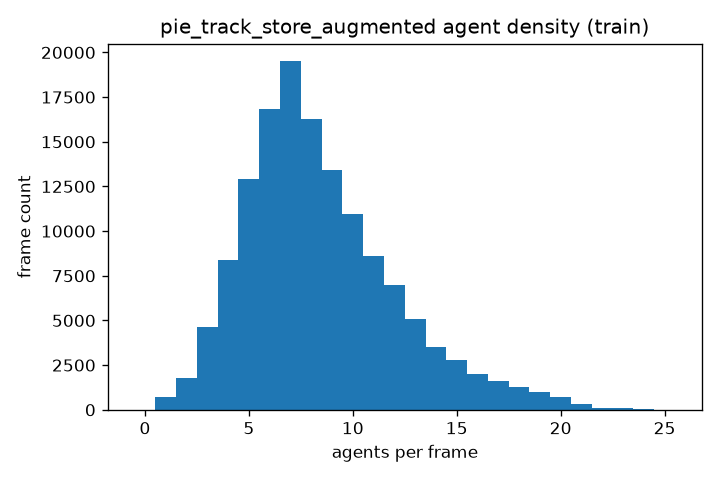
\includegraphics[width=\linewidth,height=0.13\textheight,keepaspectratio]{density_pie_track_store_augmented_train.png}
    \caption{PIE augmented (train)}
  \end{subfigure}\hfill
  \begin{subfigure}[t]{0.48\linewidth}
    \centering
    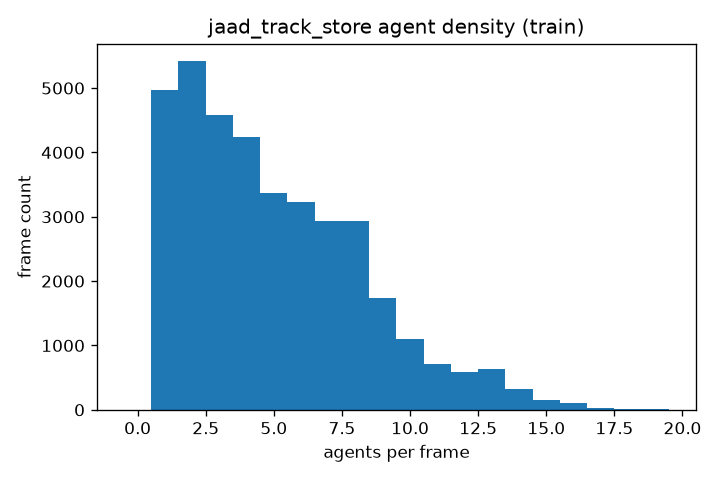
\includegraphics[width=\linewidth,height=0.13\textheight,keepaspectratio]{density_jaad_track_store_train.png}
    \caption{JAAD (train)}
  \end{subfigure}
  \caption{Agent track density per frame. Denser PIE (augmented) provides richer multi-agent context for LEMC; JAAD has sparser tracks on average.}
  \label{fig:datasets}
\end{figure}

\textbf{Backbone.}
A lightweight linear embedding followed by a 2-layer GRU predicts future bbox-centre trajectories and a binary crossing-intent logit.
The backbone is deliberately simple: capacity improvements would mask compensation effects.
All models share the same backbone; the only variation is the compensation applied to input tracks.

\textbf{Metrics.}
\begin{itemize}[leftmargin=1.2em,itemsep=1pt,topsep=2pt]
  \item \textbf{ADE/FDE}: average/final displacement error on bbox centres (pixels).
  \item \textbf{ARB/FRB@30f}: average/final relative displacement error at 30 frames, following Zhang~\textit{et al.}~\cite{zhang2024decouple}.
  \item \textbf{AUC/F1}: intent prediction area under ROC and macro F1.
  \item \textbf{Gate pass rate}: fraction of standing+moving windows satisfying $\mathrm{Var}(\text{comp})<\mathrm{Var}(\text{raw})$.
\end{itemize}
All results are mean $\pm$ std over 3 independent random seeds.
ORB extraction and detection densification are entirely offline; at inference only precomputed affines and bbox coordinates are required.

\FloatBarrier
\newpage

% ======================================================================
\section{Results}
\label{sec:results}

We report results in three steps: downstream trajectory and intent metrics on PIE and JAAD (Table~\ref{tab:main}, Fig.~\ref{fig:res_pie}), physical validity and ego-state analysis (Table~\ref{tab:diag}, Figs.~\ref{fig:res_gate}--\ref{fig:res_orb}), and cross-dataset transfer with qualitative evidence (Figs.~\ref{fig:res_jaad}--\ref{fig:res_qual}).
All numbers are mean$\pm$std over three seeds unless noted.

\textbf{Main quantitative comparison.}
Table~\ref{tab:main} summarises the full PIE grid and the JAAD transfer experiment in one place.
On PIE, fixed ORB matches the uncompensated baseline on ADE (60.5 vs.\ 60.8\,px) while improving ARB and FRB (32.3/54.5 vs.\ 34.0/56.5\,px).
This is the key trajectory result on PIE: compensation is physically correct without changing headline ADE.
Every learned LEMC variant degrades ADE by at least 21\,px, including the variant trained to regress ORB translation directly, which shows that the failure is architectural rather than due to weak supervision.
GT-speed conditioning raises intent AUC to 0.93 and F1 to 0.85, but worsens trajectory ADE to 67.0\,px, consistent with causal entanglement between driver reaction and crossing labels~\cite{lim2025tits}.
On JAAD, where no OBD signal exists, fixed ORB reduces ADE by 25\% (83.1$\rightarrow$62.7\,px) and improves all trajectory metrics while intent AUC remains at chance ($\sim$0.44).
This cross-dataset contrast is important: the same compensation is neutral where ego-motion is partially encoded in the data and strongly beneficial where it is not.

Fig.~\ref{fig:res_pie} visualises the PIE ADE ordering across all conditions and seeds.
The plot confirms that fixed ORB is the only compensation method that stays near the baseline; all LEMC variants form a separate, worse cluster.
Taken together, Table~\ref{tab:main} and Fig.~\ref{fig:res_pie} show that fixed geometry preserves PIE trajectory quality and unlocks large JAAD gains without any sensor at inference.

\begin{table*}[!t]
\centering
\caption{Main quantitative results (test set, mean$\pm$std, 3 seeds). Bold: best trajectory metric per dataset block. Italic: best intent on PIE.}
\label{tab:main}
\footnotesize
\setlength{\tabcolsep}{3.5pt}
\begin{tabular}{@{}llcccccc@{}}
\toprule
Dataset & Method & ADE & FDE & ARB & FRB & AUC & F1 \\
\midrule
\multirow{6}{*}{PIE} & Baseline & 60.8$\pm$3.3 & 121.8$\pm$9.9 & 34.0$\pm$1.4 & 56.5$\pm$4.3 & 0.89$\pm$0.01 & 0.74$\pm$0.03 \\
 & GT OBD speed & 67.0$\pm$1.3 & 136.9$\pm$3.0 & 36.2$\pm$1.8 & 59.7$\pm$2.1 & \textit{0.93$\pm$0.01} & \textit{0.85$\pm$0.02} \\
 & LEMC, no aux. & 81.7$\pm$5.1 & 159.9$\pm$2.4 & 44.2$\pm$4.4 & 70.6$\pm$3.2 & 0.77$\pm$0.05 & 0.64$\pm$0.01 \\
 & LEMC + OBD aux. & 85.8$\pm$11.2 & 164.3$\pm$11.3 & 47.4$\pm$8.2 & 73.6$\pm$6.7 & 0.80$\pm$0.01 & 0.60$\pm$0.03 \\
 & LEMC + ORB-reg. & 81.7$\pm$4.6 & 163.5$\pm$7.6 & 43.7$\pm$2.3 & 71.9$\pm$5.5 & 0.81$\pm$0.01 & 0.63$\pm$0.00 \\
 & \textbf{Fixed ORB (ours)} & \textbf{60.5$\pm$1.8} & 130.3$\pm$1.3 & \textbf{32.3$\pm$1.8} & \textbf{54.5$\pm$0.4} & 0.80$\pm$0.01 & 0.60$\pm$0.01 \\
\midrule
\multirow{2}{*}{JAAD} & Baseline & 83.1$\pm$2.0 & 156.3$\pm$4.3 & 44.8$\pm$2.2 & 71.2$\pm$2.1 & 0.47$\pm$0.05 & 0.90$\pm$0.00 \\
 & \textbf{Fixed ORB (ours)} & \textbf{62.7$\pm$2.3} & \textbf{120.1$\pm$2.8} & \textbf{34.8$\pm$2.3} & \textbf{54.2$\pm$0.9} & 0.44$\pm$0.00 & 0.90$\pm$0.00 \\
\bottomrule
\end{tabular}
\end{table*}

\begin{figure*}[!t]
  \centering
  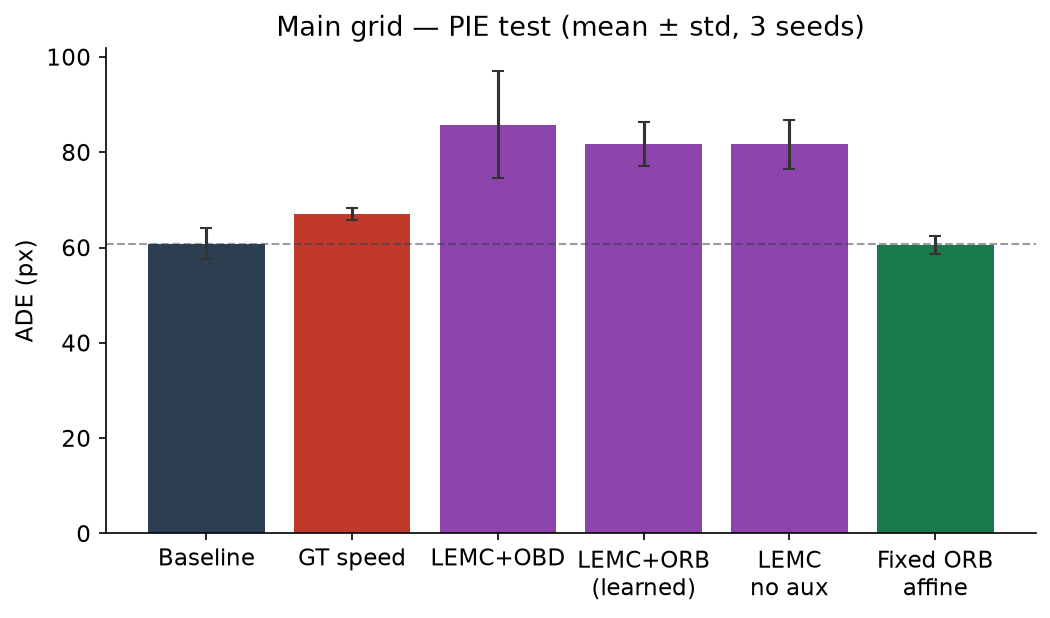
\includegraphics[width=0.92\textwidth,height=0.30\textheight,keepaspectratio]{fig_main_grid_ade.png}
  \caption{PIE ADE across all compensation conditions (3 seeds). Fixed ORB stays with the baseline cluster, while all learned LEMC variants are substantially worse. This supports the claim that only fixed geometry preserves trajectory quality on PIE.}
  \label{fig:res_pie}
\end{figure*}

\textbf{Physical validity before interpreting ADE.}
Downstream ADE alone cannot tell us whether compensation removed camera motion or introduced new distortion.
Table~\ref{tab:diag} therefore reports variance-gate pass rates together with PIE ADE stratified by ego-vehicle state.
The gate results show a clear separation: translation-only ORB passes on only $\sim$21\% of diagnostic windows, whereas per-agent full affine ORB passes $\sim$89\%.
On the full test sets, fixed ORB passes 93.1\% of standing+moving PIE windows and 96.9\% on JAAD.
By contrast, OBD-supervised LEMC passes only 0.8\% despite $R^2{=}0.30$ correlation with vehicle speed, and ORB-regression LEMC passes only 33.4\%.
The conclusion is that correlation with ego speed is not sufficient for physical validity.

The stratified ADE rows in Table~\ref{tab:diag} explain \emph{why} GT speed can look helpful in aggregate while still being harmful.
Under acceleration, GT speed yields the worst ADE (88.6\,px) while fixed ORB is best (52.2\,px).
Under deceleration, the same pattern holds (82.0 vs.\ 65.0\,px baseline).
GT speed is marginally helpful only under constant velocity.
This reproduces LIM's causal-confusion pattern~\cite{lim2025tits} on our simpler GRU backbone and shows that ego-speed input should not be treated as universally beneficial.

Fig.~\ref{fig:res_gate} makes this validity gap visible.
Panels (a--b) show that fixed ORB passes the gate on most standing+moving windows on both PIE and JAAD, while learned methods fail.
Panel (c) shows that LEMC residuals correlate with OBD speed without flattening standing pedestrians.
The important takeaway is that a method can look related to ego motion in scatter space yet still fail the physical test that matters for compensation.

\begin{table*}[!t]
\centering
\caption{Physical validity and ego-state stratification. Top: variance-gate pass rate (\%). Bottom: PIE ADE/FDE (px) by ego state (seed 0). Bold: best ADE per state.}
\label{tab:diag}
\footnotesize
\setlength{\tabcolsep}{3pt}
\begin{tabular}{@{}llcc@{}}
\toprule
\multicolumn{4}{c}{\textit{Variance gate: fraction with $\mathrm{Var}(\text{comp})<\mathrm{Var}(\text{raw})$}} \\
\midrule
Method & Scope & All (\%) & Stand.+mov.\ (\%) \\
\midrule
ORB translation only & PIE diag.\ ($n{=}300$) & \multicolumn{2}{c}{$\sim$21} \\
Per-agent full affine & PIE diag.\ ($n{=}300$) & \multicolumn{2}{c}{$\sim$89} \\
LEMC + OBD aux. & PIE test & 0.7 & 0.8 \\
LEMC + ORB-reg. & PIE test & -- & 33.4 \\
\textbf{Fixed ORB} & PIE test & \textbf{76.7} & \textbf{93.1} \\
\textbf{Fixed ORB} & JAAD test & \textbf{71.9} & \textbf{96.9} \\
\midrule
\multicolumn{4}{c}{\textit{PIE ADE / FDE by ego-vehicle state}} \\
\midrule
Ego state ($n$) & Baseline & GT speed & Fixed ORB \\
Accelerating (251) & 58.5 / 127.8 & 88.6 / 173.2 & \textbf{52.2} / \textbf{122.6} \\
Constant (1364) & 64.5 / 130.6 & \textbf{62.2} / \textbf{120.3} & 59.4 / 130.1 \\
Decelerating (158) & 65.0 / 139.8 & 82.0 / 174.7 & \textbf{67.5} / \textbf{151.5} \\
\bottomrule
\end{tabular}
\end{table*}

\begin{figure*}[!t]
  \centering
  \begin{subfigure}[t]{0.32\textwidth}
    \centering
    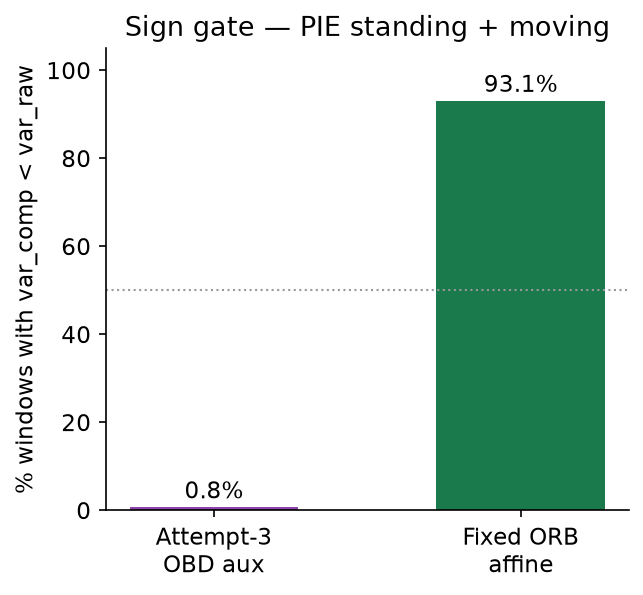
\includegraphics[width=\linewidth,height=0.28\textheight,keepaspectratio]{pie_sign_gate.png}
    \caption{PIE gate}
  \end{subfigure}\hfill
  \begin{subfigure}[t]{0.32\textwidth}
    \centering
    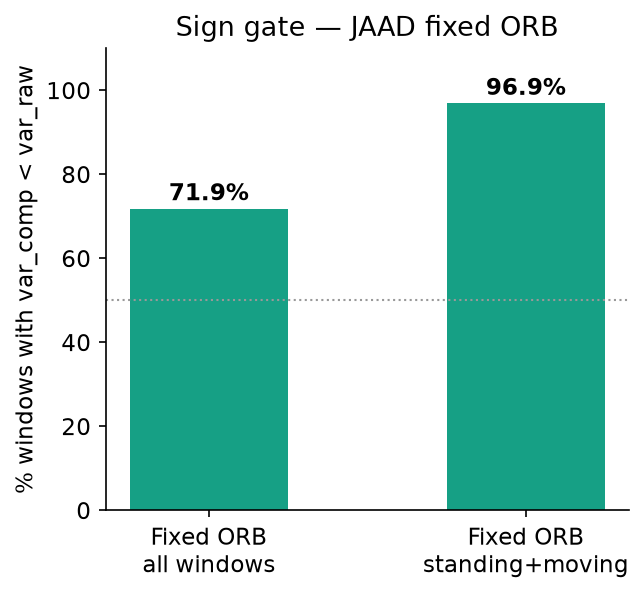
\includegraphics[width=\linewidth,height=0.28\textheight,keepaspectratio]{jaad_sign_gate.png}
    \caption{JAAD gate}
  \end{subfigure}\hfill
  \begin{subfigure}[t]{0.32\textwidth}
    \centering
    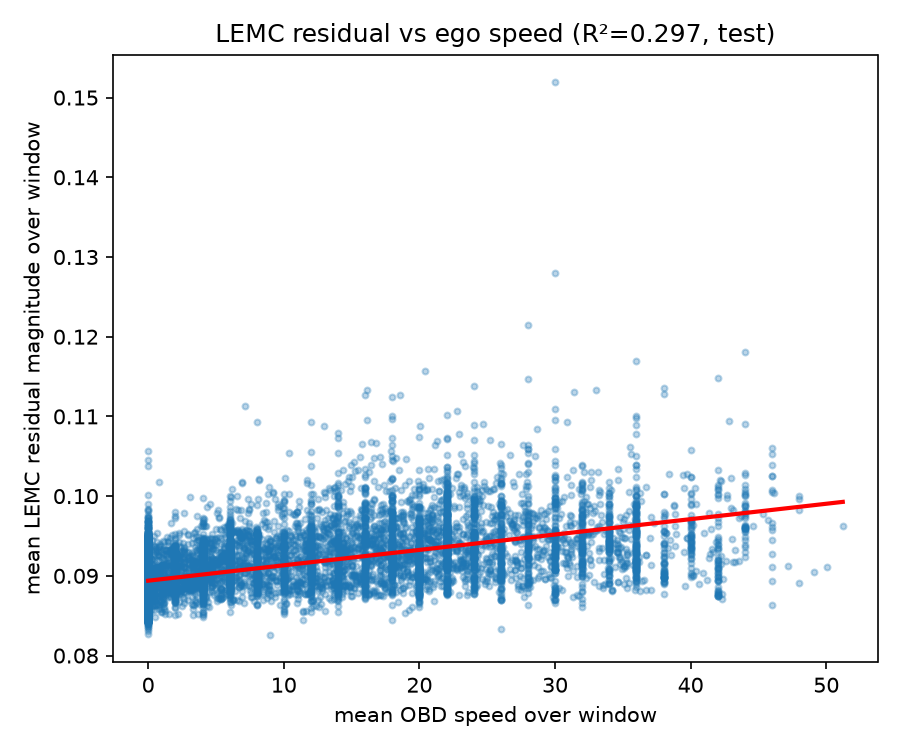
\includegraphics[width=\linewidth,height=0.28\textheight,keepaspectratio]{lemc_obd_scatter_pie_lemc_augmented_auxobd_seed0_test.png}
    \caption{LEMC vs.\ OBD}
  \end{subfigure}
  \caption{Physical validity diagnostics. (a--b) Fixed ORB passes the standing-pedestrian gate on both datasets; learned methods fail. (c) LEMC correlates with OBD ($R^2{=}0.30$) but does not produce physically valid compensation.}
  \label{fig:res_gate}
\end{figure*}

\textbf{ORB geometry validation.}
\label{sec:strat}
To verify that ORB is recovering real camera motion rather than fitting noise, Fig.~\ref{fig:res_orb}(a) plots ORB translation magnitude against OBD speed over $n{=}75{,}268$ frame pairs ($R^2{=}0.41$).
ORB never consumes speed at inference; the correlation arises because both signals reflect the same physical vehicle motion.
This supports using ORB as a sensor-free proxy for ego motion on JAAD, where OBD is unavailable.
Fig.~\ref{fig:res_orb}(b) visualises the stratified ADE pattern from Table~\ref{tab:diag}: fixed ORB is consistently strong during acceleration and deceleration, while GT speed is harmful in those regimes.
Together, these plots justify fixed ORB as a geometry-based compensator that tracks true ego motion and improves prediction where ego dynamics change quickly.

\begin{figure*}[!t]
  \centering
  \begin{subfigure}[t]{0.48\textwidth}
    \centering
    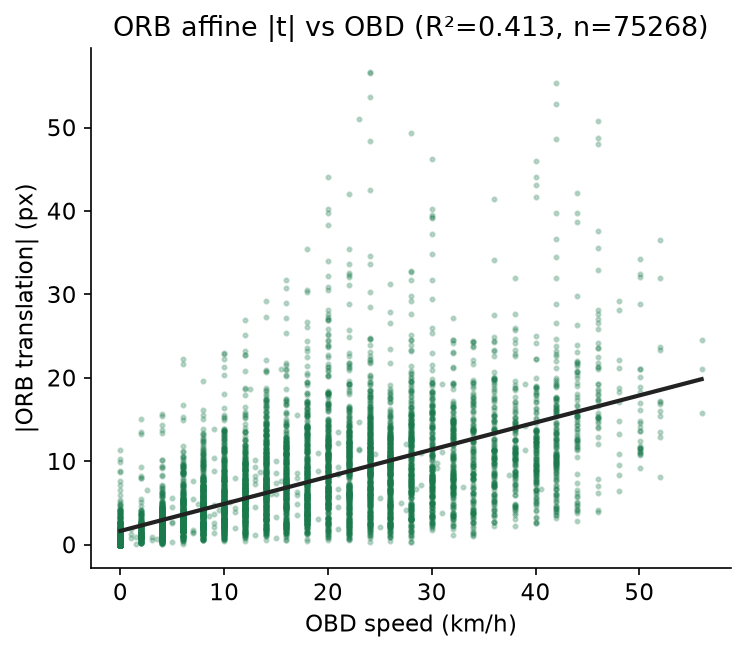
\includegraphics[width=\linewidth,height=0.30\textheight,keepaspectratio]{fig4_orb_obd_scatter.png}
    \caption{ORB $|t|$ vs.\ OBD ($R^2{=}0.41$)}
  \end{subfigure}\hfill
  \begin{subfigure}[t]{0.48\textwidth}
    \centering
    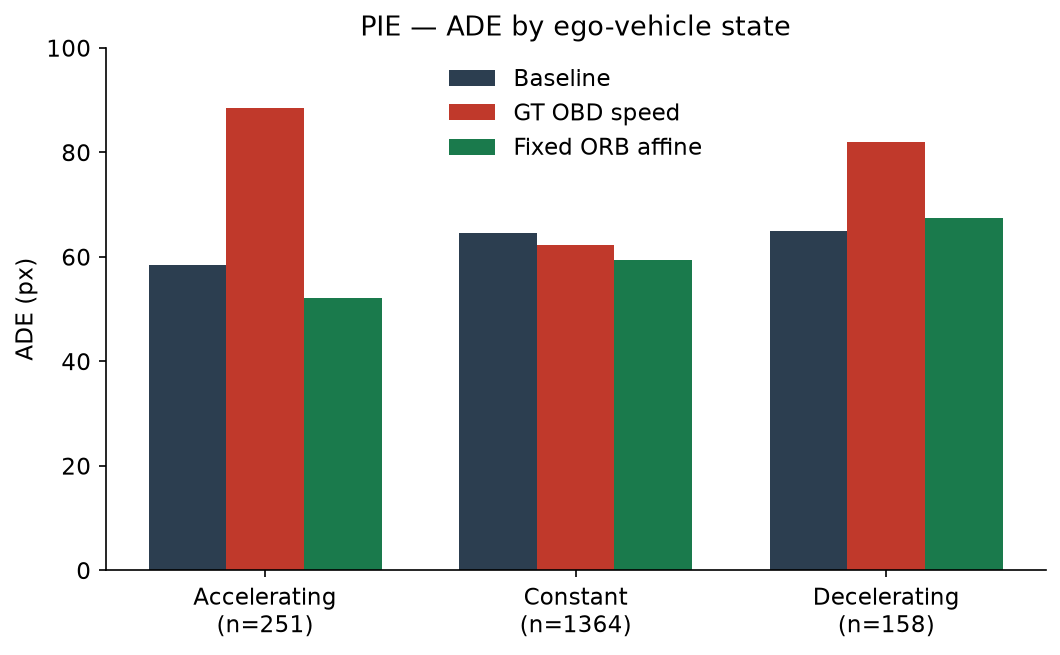
\includegraphics[width=\linewidth,height=0.30\textheight,keepaspectratio]{pie_stratified_ade.png}
    \caption{Stratified PIE ADE}
  \end{subfigure}
  \caption{ORB geometry validation and ego-state stratification. (a) ORB tracks real camera motion without a speed sensor. (b) Fixed ORB is most robust under acceleration/deceleration, where GT speed hurts most.}
  \label{fig:res_orb}
\end{figure*}

\textbf{JAAD transfer and training behaviour.}
JAAD is the deployment-relevant test because it provides no continuous ego-motion signal.
Fig.~\ref{fig:res_jaad}(a) shows that fixed ORB improves ADE, FDE, ARB, and FRB consistently across seeds.
Panels (b--c) give two representative clips where compensation collapses large baseline errors (391$\rightarrow$45\,px and 435$\rightarrow$94\,px), directly illustrating why the 25\% ADE gain in Table~\ref{tab:main} is not an aggregate artefact.
Panel (d) shows stable training with lower validation ADE for fixed ORB, confirming that the improvement is learned during training rather than a test-set fluctuation.

\begin{figure*}[!t]
  \centering
  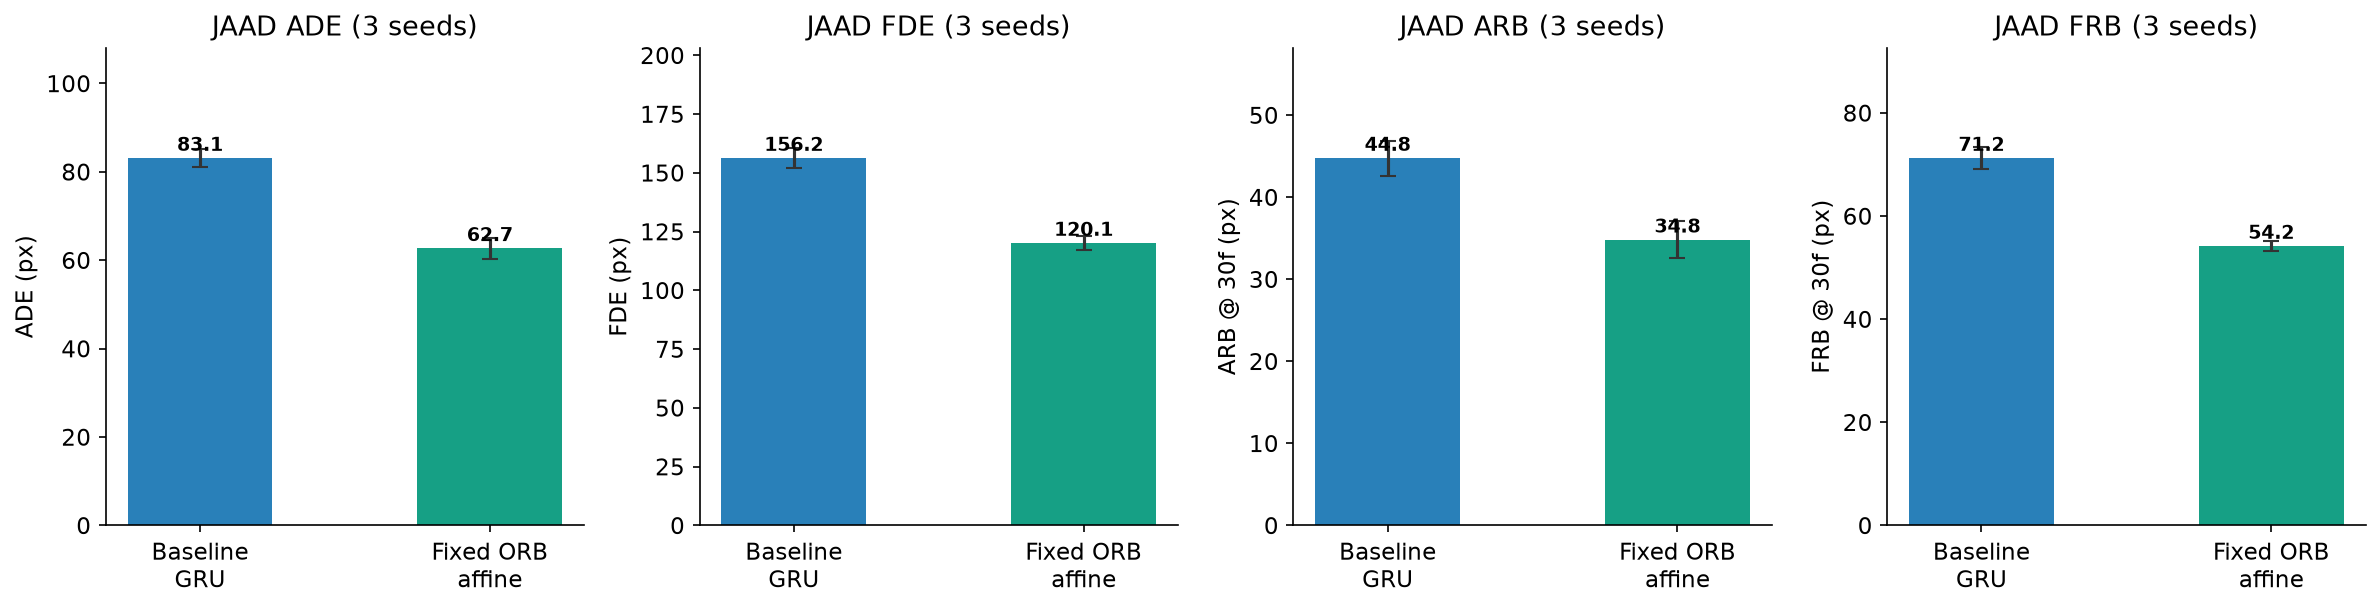
\includegraphics[width=0.95\textwidth,height=0.22\textheight,keepaspectratio]{jaad_grid_metrics.png}\\[4pt]
  \begin{subfigure}[t]{0.31\textwidth}
    \centering
    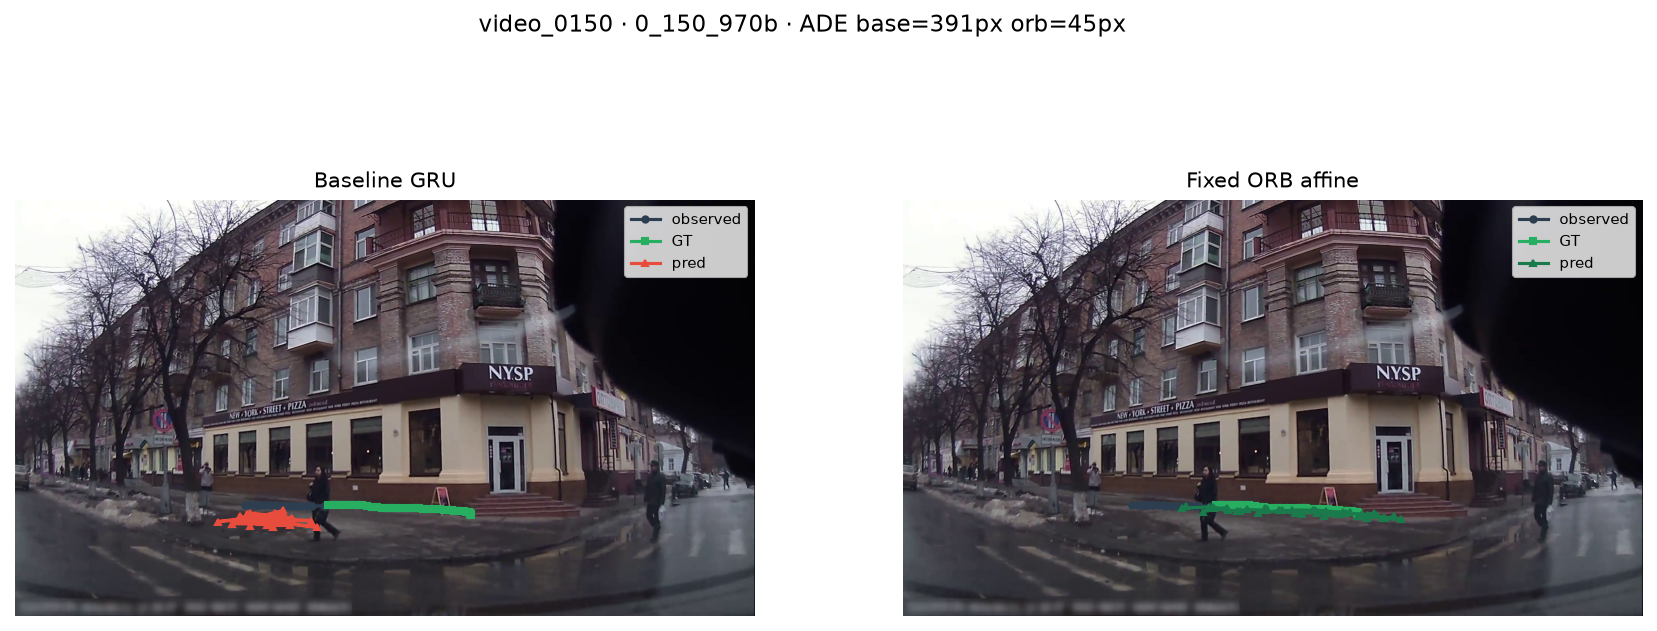
\includegraphics[width=\linewidth,height=0.26\textheight,keepaspectratio]{jaad_compare_0.png}
    \caption{Video 0150}
  \end{subfigure}\hfill
  \begin{subfigure}[t]{0.31\textwidth}
    \centering
    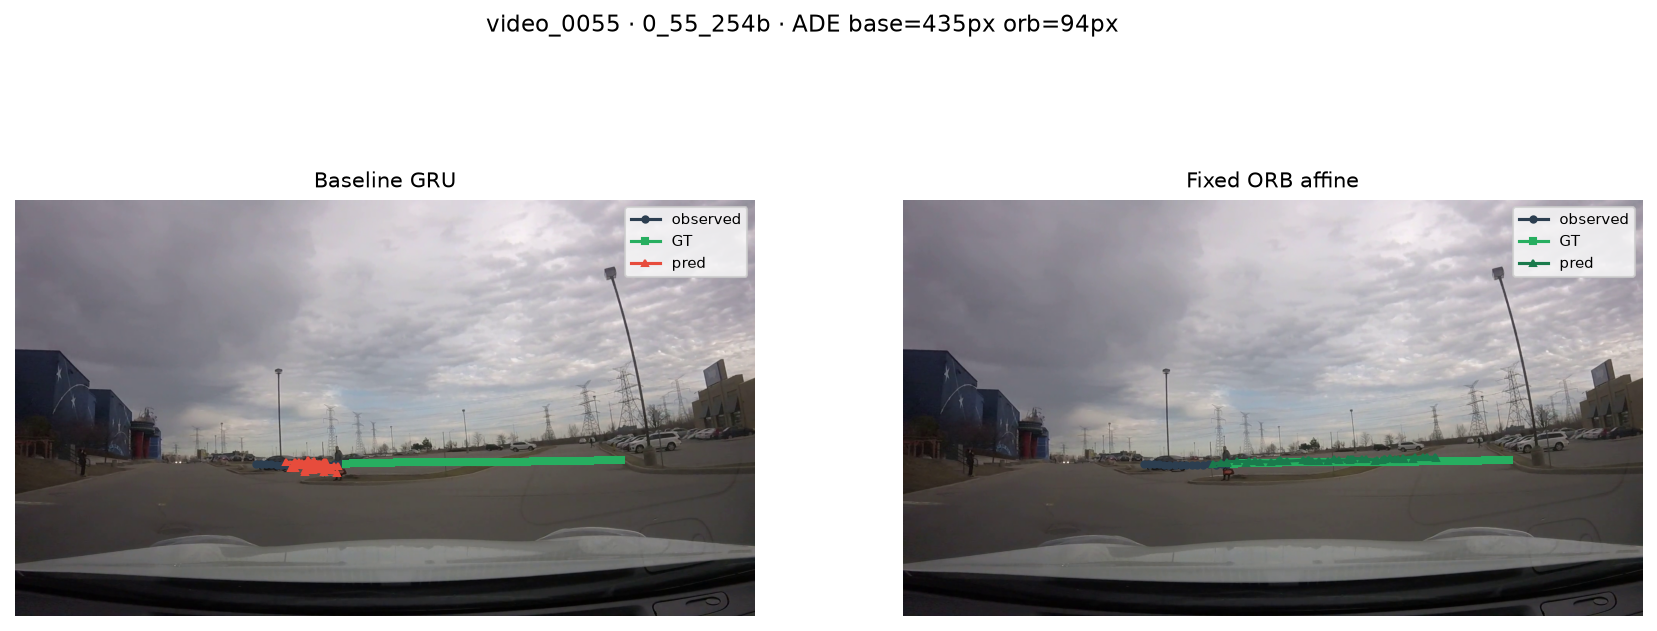
\includegraphics[width=\linewidth,height=0.26\textheight,keepaspectratio]{jaad_compare_1.png}
    \caption{Video 0055}
  \end{subfigure}\hfill
  \begin{subfigure}[t]{0.31\textwidth}
    \centering
    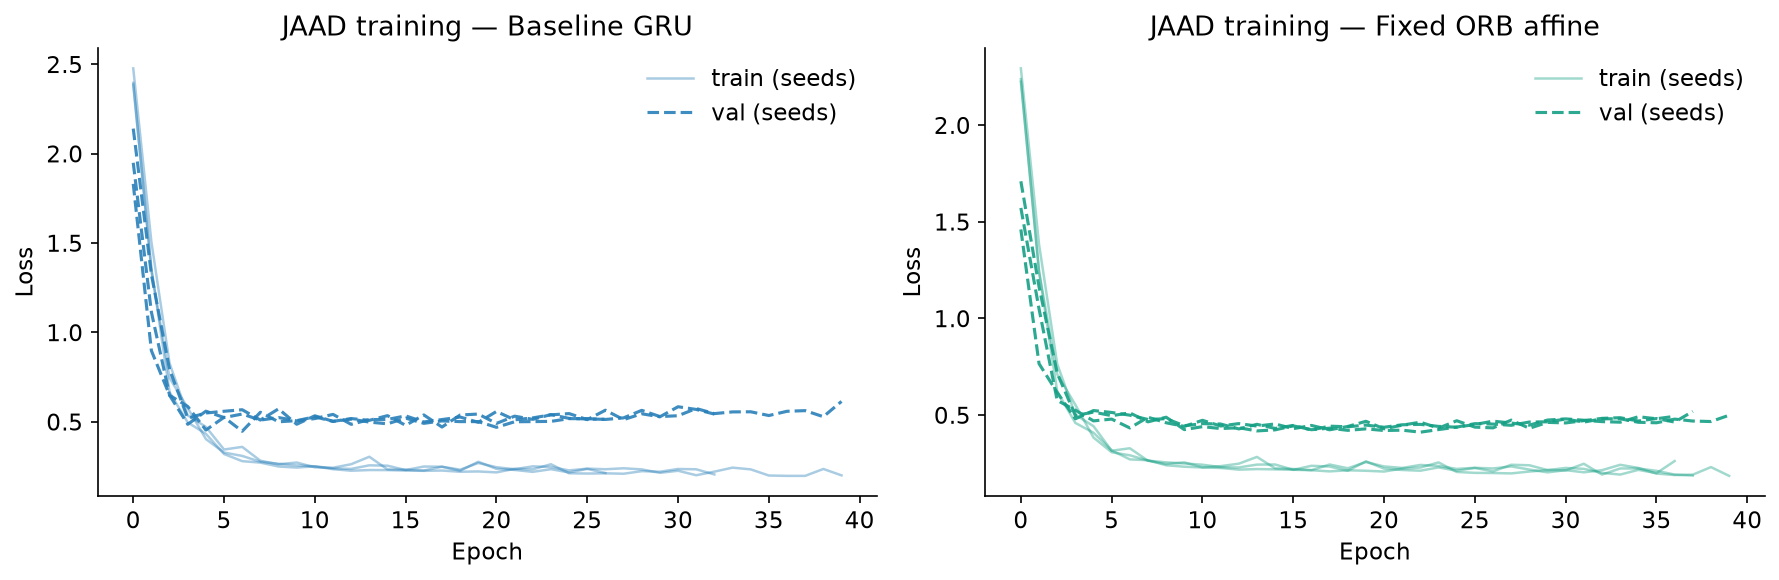
\includegraphics[width=\linewidth,height=0.26\textheight,keepaspectratio]{jaad_training_curves.png}
    \caption{Training curves}
  \end{subfigure}
  \caption{JAAD results. (a) Fixed ORB improves all trajectory metrics across seeds. (b--c) Representative overlays show large error reduction after compensation. (d) Validation ADE converges lower with fixed ORB.}
  \label{fig:res_jaad}
\end{figure*}

\textbf{Cross-dataset contrast and intent shortcut.}
Fig.~\ref{fig:res_cross} compares PIE and JAAD ADE side by side.
Fixed ORB is nearly neutral on PIE ($-$0.5\%) but improves JAAD by 25\%, showing that compensation helps most when tracks are not already partially aligned by available ego-motion cues.
Fig.~\ref{fig:res_cross}(b) reports PIE intent AUC/F1 across compensation conditions.
AUC increases monotonically with ego-motion exposure (0.80 $<$ 0.89 $<$ 0.93), and F1 follows the same order (0.60 $<$ 0.74 $<$ 0.85).
This pattern suggests that part of reported intent accuracy is driven by camera-motion cues rather than pedestrian intent alone, so trajectory and intent results should be interpreted separately after compensation.

\begin{figure*}[!t]
  \centering
  \begin{subfigure}[t]{0.48\textwidth}
    \centering
    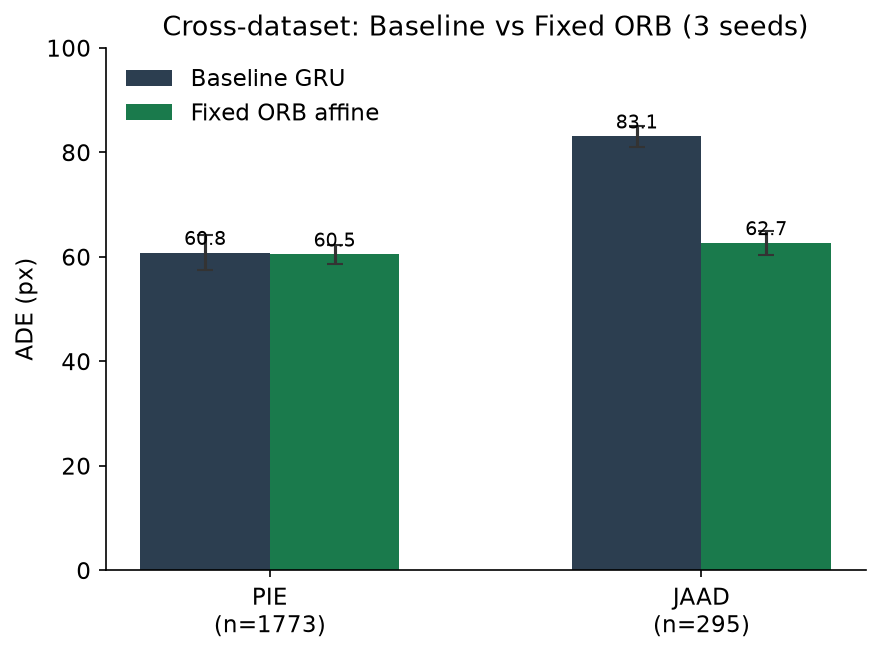
\includegraphics[width=\linewidth,height=0.30\textheight,keepaspectratio]{cross_dataset_ade.png}
    \caption{Cross-dataset ADE}
  \end{subfigure}\hfill
  \begin{subfigure}[t]{0.48\textwidth}
    \centering
    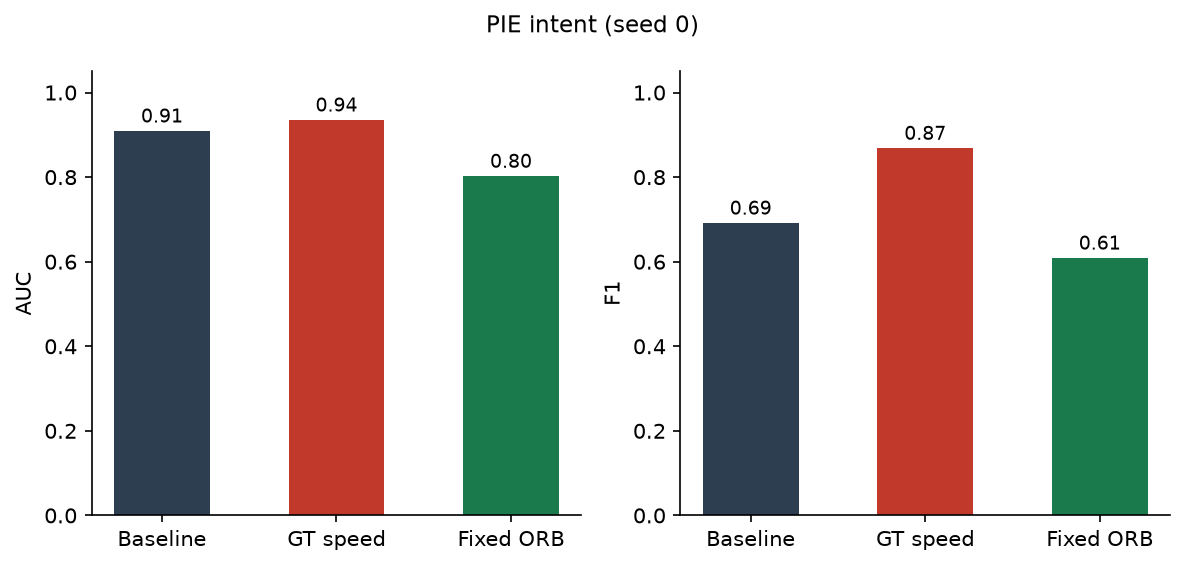
\includegraphics[width=\linewidth,height=0.30\textheight,keepaspectratio]{pie_intent_auc_f1.png}
    \caption{PIE intent AUC/F1}
  \end{subfigure}
  \caption{Cross-dataset and intent analysis. (a) Fixed ORB is neutral on PIE and strongly beneficial on JAAD. (b) Intent accuracy rises with ego-motion information, indicating a shortcut in intent evaluation.}
  \label{fig:res_cross}
\end{figure*}

\textbf{Qualitative evidence.}
Fig.~\ref{fig:res_qual} provides four complementary views of the same conclusions.
Panel (a) shows a standing pedestrian at 18.6\,km/h: raw tracks drift while compensated tracks remain near stationary, confirming the variance gate visually.
Panel (b) shows a PIE overlay where compensated prediction follows pedestrian motion more faithfully.
Panel (c) shows that LEMC correlates with OBD speed without producing valid flattening.
Panel (d) shows a failure mode where the learned residual loops instead of removing camera motion.
These examples explain why fixed ORB is preferred over learned residuals despite similar apparent correlations in some plots.

\begin{figure*}[!t]
  \centering
  \begin{subfigure}[t]{0.48\textwidth}
    \centering
    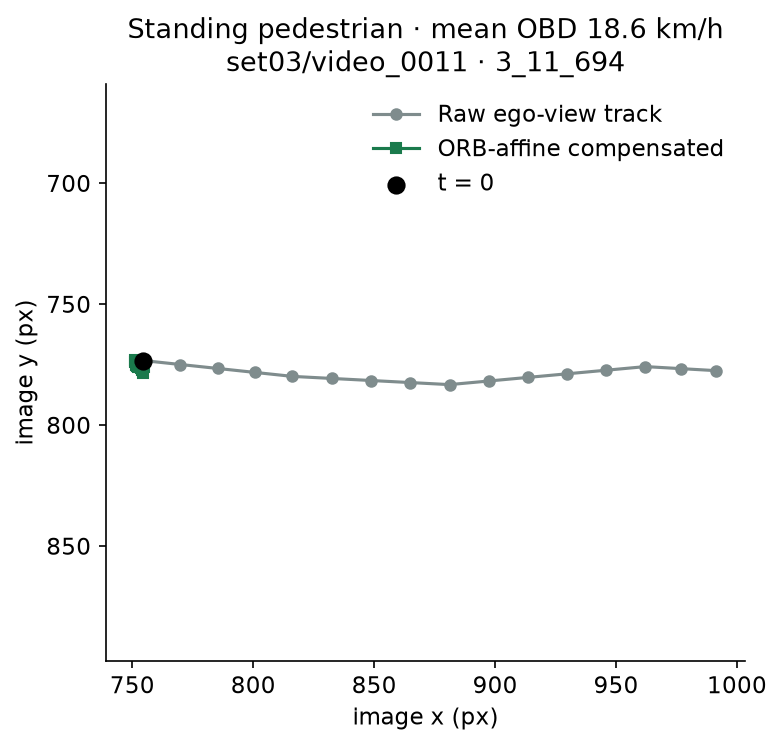
\includegraphics[width=\linewidth,height=0.28\textheight,keepaspectratio]{fig1_teaser.png}
    \caption{Standing pedestrian}
  \end{subfigure}\hfill
  \begin{subfigure}[t]{0.48\textwidth}
    \centering
    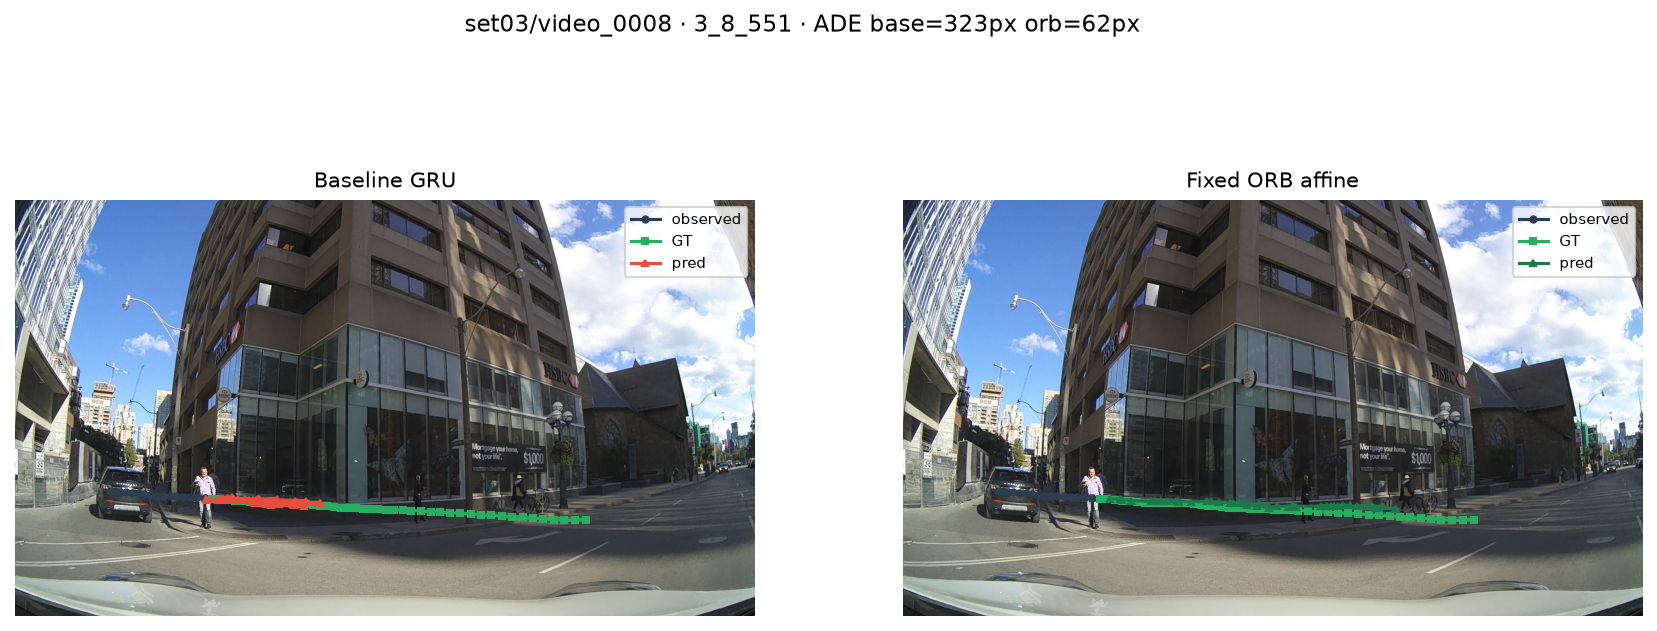
\includegraphics[width=\linewidth,height=0.28\textheight,keepaspectratio]{pie_compare_0.png}
    \caption{PIE overlay}
  \end{subfigure}\\[4pt]
  \begin{subfigure}[t]{0.48\textwidth}
    \centering
    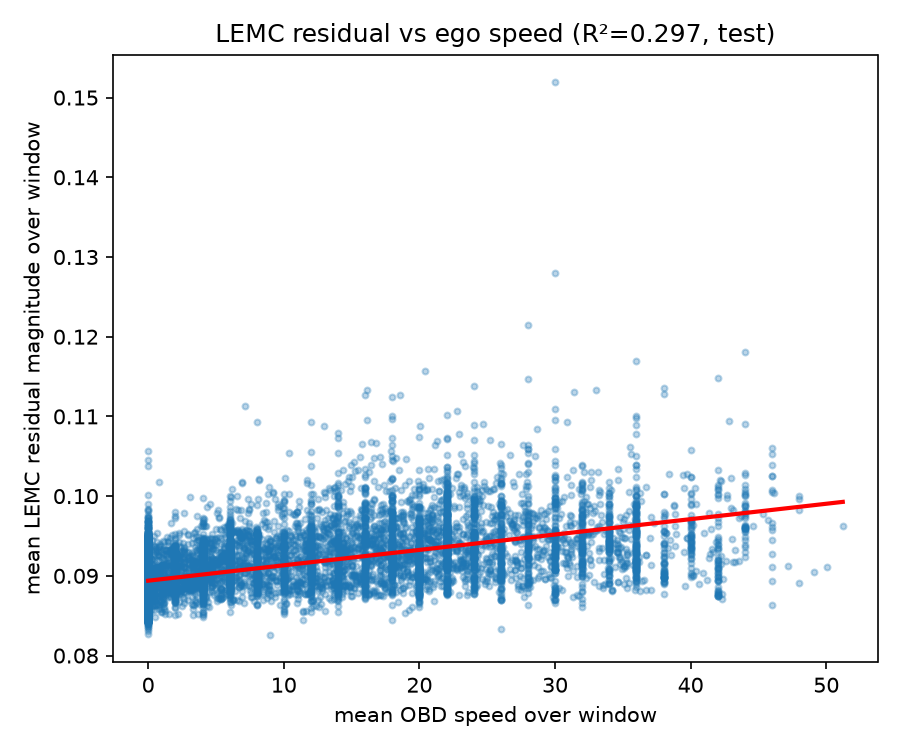
\includegraphics[width=\linewidth,height=0.28\textheight,keepaspectratio]{lemc_obd_scatter_pie_lemc_augmented_auxobd_seed0_test.png}
    \caption{LEMC--OBD correlation}
  \end{subfigure}\hfill
  \begin{subfigure}[t]{0.48\textwidth}
    \centering
    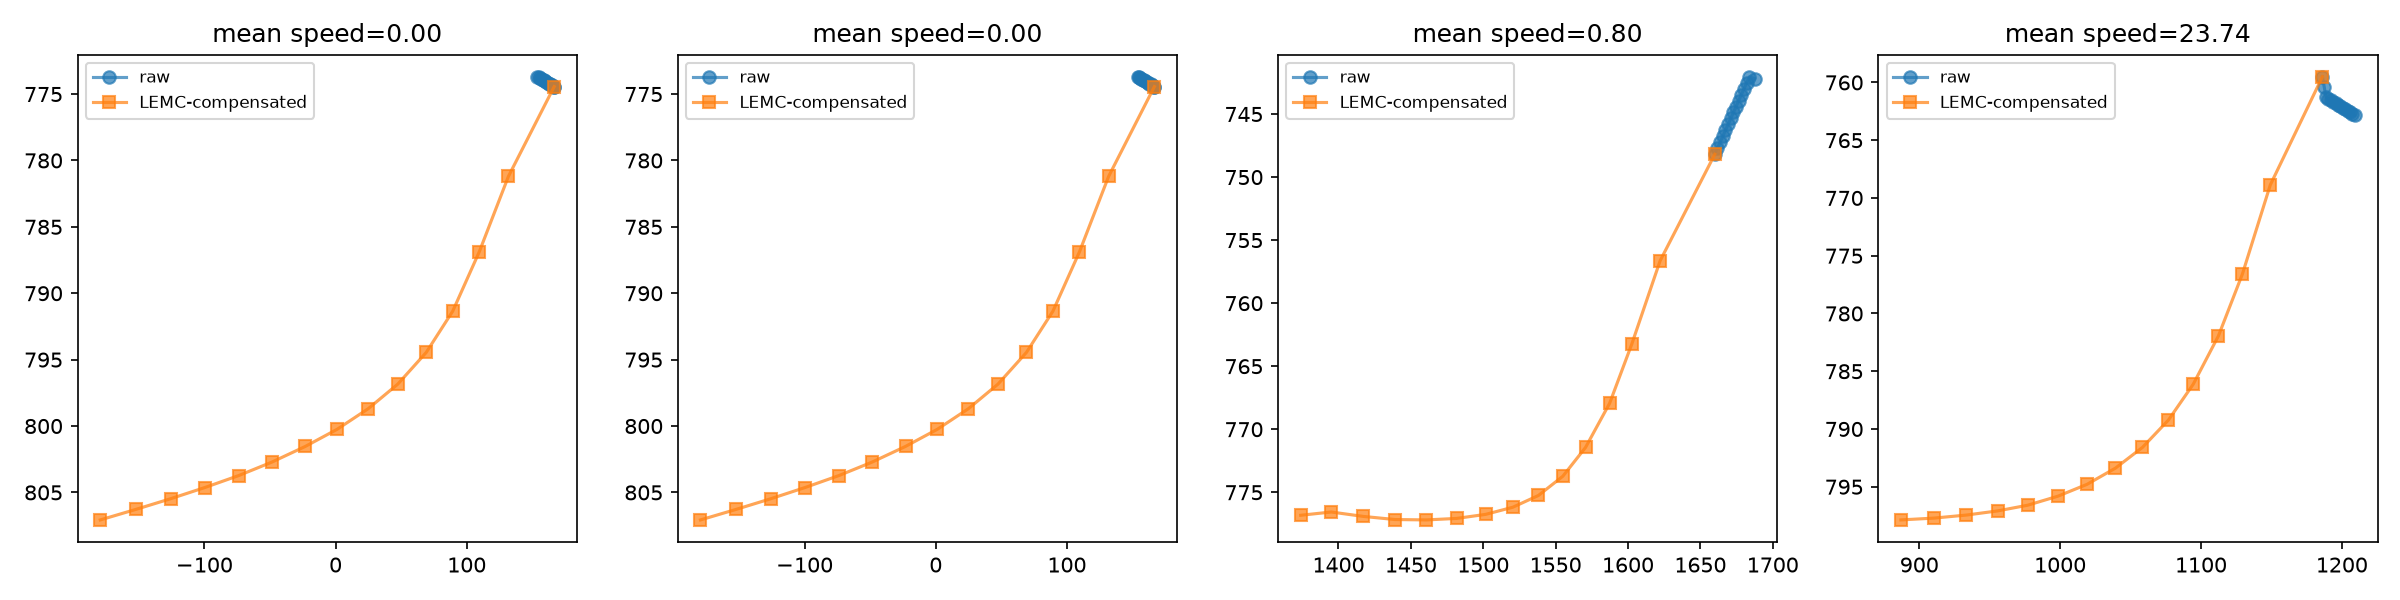
\includegraphics[width=\linewidth,height=0.28\textheight,keepaspectratio]{lemc_qualitative_pie_lemc_augmented_auxobd_seed0_test.png}
    \caption{LEMC failure mode}
  \end{subfigure}
  \caption{Qualitative results. (a) Valid ORB flattening of standing-pedestrian drift. (b) Improved PIE trajectory overlay. (c) Correlation without physical validity. (d) Learned residual failure (looping).}
  \label{fig:res_qual}
\end{figure*}

\FloatBarrier

% ======================================================================
\section{Discussion}
\label{sec:discussion}

\textbf{Why does fixed geometry outperform learned residuals?}
A global 2-D shift cannot capture rotation and scale, whose apparent effect depends on image-plane position.
Multi-agent displacement statistics aggregate over pedestrians at different positions, so the learned residual fits a mean across inconsistent targets.
ORB-regression supervision does not resolve this: even when directly trained to predict ORB translations, LEMC fails the gate (33.4\%).
The failure mode is architectural, not data-limited.
This parallels Azarmi~\textit{et al.}'s~\cite{azarmi2024feature} finding that training-time correlation with a target is insufficient if the underlying physical process is not correctly represented.

\textbf{Why is PIE neutral while JAAD improves?}
On PIE, drivers typically reduce speed before pedestrians cross, creating a spurious statistical alignment between ego motion and pedestrian trajectory.
The uncompensated baseline already benefits from this alignment (the pedestrian is crossing while the car slows, reducing ego drift).
Fixed ORB removes this confound, leaving ADE essentially unchanged.
On JAAD, with no such OBD-mediated pre-alignment and higher vehicle speeds in some clips, raw tracks carry more uncompensated ego drift; removing it yields substantial ADE improvement.
This dissociation strengthens the causal argument: the gain is not due to compensation quality alone, but to the presence or absence of latent OBD alignment in the uncompensated tracks.

\textbf{Intent shortcut implications.}
The monotonic AUC ordering (0.80 $<$ 0.89 $<$ 0.93) across all PIE conditions suggests that intent AUC is partially inflated by ego-motion correlation rather than purely reflecting pedestrian intent.
Future intent benchmarks should either (a) evaluate after explicit ego-motion removal or (b) stratify by vehicle state to isolate pedestrian-specific variation.

\textbf{Limitations.}
Our backbone is a deliberately simple GRU on bbox coordinates.
ORB affine quality is degraded by depth variation (a scene-level depth confound caps $R^2$ at 0.41).
Missing affines (featureless frames) are imputed by holding the last valid affine.
JAAD intent AUC stays at chance because the dataset does not provide matched crossing labels per clip in our protocol.
Shortcut isolation relies on the variance gate rather than a dedicated causal intervention.

% ======================================================================
\section{Conclusion}
\label{sec:conclusion}

We showed that offline position-dependent ORB affine compensation passes a physical standing-pedestrian variance gate that three learned alternatives fail, while remaining trajectory-neutral on PIE ($-$0.5\% ADE) and improving JAAD by 25\% (20\,px absolute), with zero ego-motion sensors required at inference.
Intent AUC tracks available ego-motion (0.80 $\rightarrow$ 0.89 $\rightarrow$ 0.93): trajectory and intent benchmarks carry different information after compensation and should be reported separately.
The variance gate is a cheap, training-free filter that any proposed learned ego-motion module should pass before downstream evaluation; fixed offline geometry already does.
Configs, ORB extraction scripts, and three-seed checkpoints are released to support reproducible comparison on JAAD, a dataset that exposes ego-motion shortcuts invisible when OBD labels are always available.

\bibliographystyle{IEEEtran}
\bibliography{refs}

\end{document}
